\section{Working with the data and calculating the time peiod}

\subsection{Finding Time Period in Lab frame}

	We got the data in the form of two arrays, one with the time (in milliseconds) and the other with the value of the photo-transistor in volts (0 to 5V). We thought it would be easier for us to work with digital data. So we changed the array to only \texttt{True} and \texttt{False} values with a threshold of 3V.

	We decided to call it a peak when we see a \texttt{True} value followed by a \texttt{False} value (i.e: we are detecting when it is going down every time any other point like when it is going up could have worked as well). We first find the first peak, and store the time to a variable $t_0$. Then we move along the graph, and when we found the next peak, we found the difference between the time of this peak and $t_0$. Thus we got the distance between these consecutive peaks.

	Next we store the time of the current peak to $t_0$ and move forward to find the next peak. We repeat this process until we find all the peaks and store the time difference between consecutive peaks in an array.

	\vspace{3mm}

	\noindent \textbf{Problem Faced:} We found that, the time difference between consecutive peaks was not constant always. Two peaks sometimes have a tendency to come closer. We need to remember that the pendulum crosses the mean position twice in one oscillation. So, if the detector is not present exactly in the mean position, we will have unequal angles to swing on the left and the right. So, although the time difference between every $odd^{th}$ peak and every $even^{th}$ peak is same, the time between two consecutive peaks don't remain same.

	To avoid this issue, we decided to consider only even number of differences into consideration. Thus, if we took $2n$ differences, we will get $n$ oscillation data (apart from two of the extreme points, in one oscillation a pendulum crosses every other point in the path twice). This was achieved by removing the last element of the list if the length of the list was odd.

	Now the array was in milliseconds, and contained distances between consecutive peaks. So, we took the average of the array and multipled it by (1000/2) = 500. This gave us the average time period of the oscillation.
	
	\begin{lstlisting}[language=Python, caption={Python code to find the time period of the oscillation.}, label={code:time_period}]
def times_between_peaks(t, val):
	val = val > 3  # converting to binary values

	i = 0 # index of t
	got_first = False
	ts = []
	while i < len(val)-1:
		# finding the first peak is important
		if not got_first:
			if val[i] == True and val[i+1] == False:
				t0 = t[i]
				got_first = True  # first peak found
		else:
			if val[i] == True and val[i+1] == False:
				ts.append(t[i] - t0)
				t0 = t[i]
		i += 1

	# removing the last peak if oscillations are not complete
	if len(ts)%2: ts.pop()  # if len(ts) is odd
	return np.array(ts)  # in milliseconds

# CALLING THE FUNCTION: we had taken the data before in variables t and val
times = times_between_peaks(t, val)
T = times.mean()/500  # time period in seconds \end{lstlisting}

\subsection{Finding acceleration of lift}
	
	While calculating the acceleration in lift, we found that the acceleration was not uniform. So, we decided to take the maximum acceleration recorded from all the 6 trials and to take the average. \textbf{In \hyperref[th:4]{Figure 4} we can see one of the 6 data points we recorded (one data point corresponds to whole data of  going up to 4th floor from Ground floor in one of the SPS lifts)}

	\begin{figure}
		\centering
		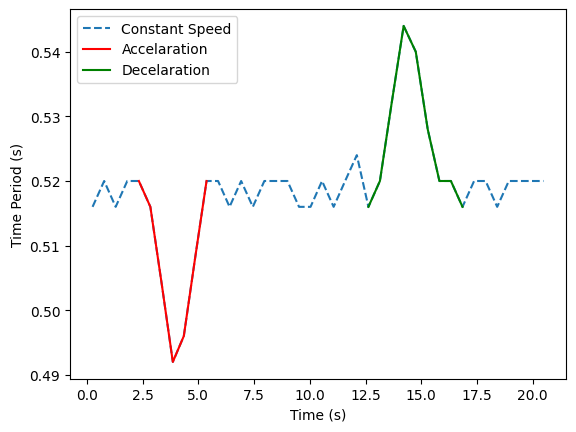
\includegraphics[width=0.75\columnwidth]{images/example_graph2.png}
		\caption{Graph of the time period variations in lift}
		\label{th:4}
	\end{figure}